\documentclass[a4paper,french,bookmarks]{article}
\usepackage{./Structure/4PE18TEXTB}

\renewcommand{\thesection}{\Roman{section}} 
\begin{document}
\stylizeDoc{Physique}{Devoir Maison 7}{La matinée d'Albert}
\newboxans

On s'intéresse à la matinée typique d'un physicien, Albert.\\[-15pt]
%
\begin{center}
    \itshape Les parties de ce problème sont indépendantes.
\end{center}

\section{Albert prend une douche}

Commençons par quelques considérations générales. L'air renferme toujours une proportion d'eau sous forme vapeur. On le qualifie d'air humide et on le caractérise par
% Curieux, besoin de cet espace vide pour que le premier que "triangle" de l'enum 
% s'affiche
\hfill
%
\begin{minipage}{0.35\linewidth}
	\centering
	\begin{tabular}{c|c}
	\end{tabular}
\end{minipage}
%
\begin{enumerate}
	\itt son \textit{humidité absolue} :
    
    \begin{equation}
        x = \dfrac{m_\text v}{m_\text{as}}
    \end{equation}
    
    où $m_\text v$ et $m_\text{as}$ sont respectivement les masses de vapeur d'eau et d'air sec dans un volume $V$ quelconque d'air humide ;
    
    \itt son \textit{humidité relative} $H_\text r$ (ou \textit{degré hydrométrique}, ou \textit{taux d'humidité}) à la température $T$ :
    
    \begin{equation}
        H_\text{r} = \dfrac{p_\text{v}}{p_\text{sat}\left(T\right)}
    \end{equation}
    
    où $p_\text v$ est la pression partielle en vapeur d'eau et $p_\text{sat}$ la pression de vapeur saturante dont la dépendance avec la température est donnée par la figure \ref{fig:fig1}. On dit que l'air est saturé si $H_\text{r} = 1$.
\end{enumerate}

Dans la suite, l'air humide sera étudié comme un mélange de deux gaz parfaits : l'air sec (indice \guill{as}) et la vapeur
d'eau (indice \guill{v}). La pression totale $p$ de l'air humide sera considérée constante et égale à $p = \SI{1.013}{\bar}$.
%
On note respectivement $M_\text{as}$ et $M_e$ les masses molaires de l'air sec et de l'eau.

\begin{figure}[h]
	\centering
    \begin{tikzpicture}
        \begin{axis}[
            axis lines = left,
            xlabel=$T \ \left(\SI{}{\celsius}\right)$,
            ylabel=$p_\text{sat} \ \left(\SI{}{\pascal}\right)$,
            domain=0:25,
            log basis x={10},
            xmin=0,
            xmax=25,
            ymin=500,
            ymax=3000,
            xtick distance=5,
            ytick distance=500,
            minor x tick num=4,
            minor y tick num=4,
            grid = major,
            grid style = {line width = .1pt, draw = gray!30},
            major grid style = {line width=.2pt,draw=gray!50}
        ]
            \addplot[color=main1, line width=0.4mm, smooth,samples=200]{611.21*exp((18.678-x/234.5)*(x/(257.14+x)))};
            
            \draw[dotted, very thick] (0, 2338) -- (20, 2338) -- (20, 0);
            
            \draw[dotted, very thick] (0, 1228) -- (10, 1228) -- (10, 0);
        \end{axis}
    \end{tikzpicture}
	\caption{Pression de vapeur saturante en fonction de la température.}
	\label{fig:fig1}
\end{figure}

\begin{enumerate}
    \item Estimer les valeurs numériques de $M_\text{as}$ et $M_\text{e}$.
    
    \boxans{
        En première approximation, l'air sec est constitué à \SI{80}{\percent} de diazote $\left(\text N_2\right)$ et à \SI{20}{\percent} de dioxygène $\left(\text O_2\right)$. Le diazote est de masse molaire $M_{\text N_2} = 2M_\text N \approx 2\times 14,0 = \SI{28,0}{\g \cdot \mol^{-1}}$, et le dioxygène est de masse molaire $M_{\text O_2} = 2M_\text O \approx 2\times 16,0 = \SI{32,0}{g \cdot \mol^{-1}}$. On a alors $M_\text{as} = 0,8M_{\text N_2} + 0,2M_{\text O_2}$. On obtient $M_\text{as} = \SI{28,8}{\g \cdot \mol^{-1}}$.
        
        L'eau $\left(\text H_2 \text O\right)$ est de masse molaire $M_\text e = 2M_\text H + M_\text O$. On obtient $M_\text e = \SI{18.0}{\g \cdot \mol^{-1}}$.
    }
    
    \item Montrer que
    
    \begin{equation}
        x = d \dfrac{p_\text v}{p - p_\text v} \qquad\text{où}\qquad d = \dfrac{M_\text e}{M_\text{as}}
    \end{equation}
    
    \boxans{
        On note respectivement $n_\text{as}$ et $n_\text e$ les quantités de matière d'air sec et d'eau et $p_\text{as}$ la pression partielle de l'air sec. Le système est \{ air sec + vapeur d'eau \} donc $p = p_\text{v} + p_\text{as}$ soit $p_\text{as} = p - p_\text e$.
    }
    
    \boxans{
        On a $m_\text i = n_\text iM_\text i$ donc $x = \dfrac{M_\text en_\text e}{M_\text{as}n_\text{as}} = d\dfrac{n_\text e}{n_\text{as}}$. On suppose alors que la vapeur d'eau et l'air sec sont des gaz parfaits. La loi du même nom livre $n_\text i = p_\text i \dfrac{V}{RT}$, d'où $x = d\dfrac{p_\text v}{p_\text{as}}$ donc finalement $x = d \dfrac{p_\text v}{p - p_\text v}$.
    }
    
    \item Calculer la valeur maximale de l'humidité absolue $x_\text{sat}$ de l'air humide à la température $T_0 = \SI{20}{\celsius}$.
    
    \boxans{
        Si l'humidité absolue est maximale, alors on a atteint la pression de vapeur saturante $p_\text{sat}\left(T_0\right)$. On lit graphiquement $p_\text = p_\text{sat}\left(T_0\right) = \SI{2350}{\pascal}$. En appliquant la formule précédente, on obtient $x_\text{sat} = 1.48$.
    }
\end{enumerate}

Albert décide de prendre une douche. Le volume intérieur de sa salle de bain est $V = \SI{15}{\m^3}$ et l'humidité relative initiale est $H_\text {r,i} = \SI{50}{\percent}$. On note $T_\text i = \SI{20}{\celsius}$ la température intérieure de la salle de bain, et $T_\text e = \SI{10}{\celsius}$ la température de l'air à l'extérieur du logement.\\[2pt]
%
Un miroir est encastré dans le mur de la salle de bain qui donne directement sur l'extérieur. La température de la surface du miroir ainsi que celle du mur dans lequel il est encastré est de $T_\text S = \SI{14}{\celsius}$.

\begin{enumerate}[resume]
    \item Expliquer qualitativement pourquoi la température de surface du miroir est inférieure à la température de l'air dans la pièce.
    
    \boxans{
        Le miroir est encastré dans le mur qui agît comme une interface entre l'intérieur de la pièce, à la température $T_\text i$, et l'extérieur du logement, à la température $T_\text e < T_\text i$. Sa température se situe donc entre les deux, approximativement vers le milieu, ce seuil variant selon différents facteurs lié à la conduction thermique du mur. 
    }
\end{enumerate}

Le \textit{point de rosée} ou \textit{température de rosée} est la température la plus basse à laquelle une masse d'air peut être soumise, à pression et humidité données, sans qu'il se produise une formation d'eau liquide par saturation, ce qu'on appelle \textit{condensation} ou simplement \guill{buée}. La figure \ref{fig:fig2} donne le point de rosée en fonction de la température de l'air pour différents niveaux d'humidité relative. On voit par exemple sur le graphe que pour un air à \SI{25}{\celsius} d'humidité relative égale à \SI{40}{\percent}, de la buée apparaît si cet air est en contact avec une surface de température inférieure à \SI{10}{\celsius}.

\begin{figure}[h]
	\centering
    \begin{tikzpicture}
        \begin{axis}[
            axis lines = left,
            xlabel={Température de l'air $T_\text a \ \left(\si{\celsius}\right)$},
            ylabel={Point de rosée $T_\text r \ \left(\si{\celsius}\right)$},
            domain=0:25,
            log basis x={10},
            xmin=0,
            xmax=40,
            ymin=0,
            ymax=40,
            xtick distance=5,
            ytick distance=5,
            minor x tick num=4,
            minor y tick num=4,
            grid = major,
            grid style = {line width = .1pt, draw = gray!30},
            major grid style = {line width=.2pt,draw=gray!50}
        ]
            \draw[main1!90!main3] (0, 0.0) -- (1, 1.0) -- (2, 2.0) -- (3, 3.0) -- (4, 4.0) -- (5, 5.0) -- (6, 6.0) -- (7, 7.0) -- (8, 8.0) -- (9, 9.0) -- (10, 10.0) -- (11, 11.0) -- (12, 12.0) -- (13, 13.0) -- (14, 14.0) -- (15, 15.0) -- (16, 16.0) -- (17, 17.0) -- (18, 18.0) -- (19, 19.0) -- (20, 20.0) -- (21, 21.0) -- (22, 22.0) -- (23, 23.0) -- (24, 24.0) -- (25, 25.0) -- (26, 26.0) -- (27, 27.0) -- (28, 28.0) -- (29, 29.0) -- (30, 30.0) -- (31, 31.0) -- (32, 32.0) -- (33, 33.0) -- (34, 34.0) -- (35, 35.0) -- (36, 36.0) -- (37, 37.0) -- (38, 38.0) -- (39, 39.0) -- (40, 40.0); %Hr: 100
            
            \node[rotate=43] at (20,22) {\color{main1!90!main3}\small$\SI{100}{\percent}$};
            
            \draw[main1!80!main3] (0, -1.3) -- (1, -0.4) -- (2, 0.5) -- (3, 1.5) -- (4, 2.5) -- (5, 3.5) -- (6, 4.5) -- (7, 5.5) -- (8, 6.4) -- (9, 7.5) -- (10, 8.4) -- (11, 9.4) -- (12, 10.4) -- (13, 11.4) -- (14, 12.4) -- (15, 13.4) -- (16, 14.4) -- (17, 15.3) -- (18, 16.3) -- (19, 17.3) -- (20, 18.3) -- (21, 19.3) -- (22, 20.3) -- (23, 21.3) -- (24, 22.3) -- (25, 23.2) -- (26, 24.2) -- (27, 25.2) -- (28, 26.2) -- (29, 27.2) -- (30, 28.2) -- (31, 29.2) -- (32, 30.1) -- (33, 31.1) -- (34, 32.1) -- (35, 33.1) -- (36, 34.1) -- (37, 35.1) -- (38, 36.1) -- (39, 37.1) -- (40, 38.0); %Hr: 90
            
            \draw[main1!70!main3] (0, -3.1) -- (1, -2.0) -- (2, -0.9) -- (3, -0.1) -- (4, 0.8) -- (5, 1.9) -- (6, 2.8) -- (7, 3.8) -- (8, 4.7) -- (9, 5.8) -- (10, 6.7) -- (11, 7.7) -- (12, 8.6) -- (13, 9.6) -- (14, 10.6) -- (15, 11.6) -- (16, 12.6) -- (17, 13.5) -- (18, 14.5) -- (19, 15.5) -- (20, 16.4) -- (21, 17.4) -- (22, 18.4) -- (23, 19.4) -- (24, 20.3) -- (25, 21.3) -- (26, 22.3) -- (27, 23.2) -- (28, 24.2) -- (29, 25.2) -- (30, 26.2) -- (31, 27.1) -- (32, 28.1) -- (33, 29.1) -- (34, 30.0) -- (35, 31.0) -- (36, 32.0) -- (37, 33.0) -- (38, 33.9) -- (39, 34.9) -- (40, 35.9); %Hr: 80
            
            \draw[main1!60!main3] (0, -5.1) -- (1, -4.0) -- (2, -3.0) -- (3, -1.9) -- (4, -0.8) -- (5, 0.0) -- (6, 0.9) -- (7, 1.9) -- (8, 2.8) -- (9, 3.9) -- (10, 4.8) -- (11, 5.7) -- (12, 6.7) -- (13, 7.6) -- (14, 8.6) -- (15, 9.6) -- (16, 10.5) -- (17, 11.5) -- (18, 12.4) -- (19, 13.4) -- (20, 14.4) -- (21, 15.3) -- (22, 16.3) -- (23, 17.2) -- (24, 18.2) -- (25, 19.1) -- (26, 20.1) -- (27, 21.1) -- (28, 22.0) -- (29, 23.0) -- (30, 23.9) -- (31, 24.9) -- (32, 25.8) -- (33, 26.8) -- (34, 27.7) -- (35, 28.7) -- (36, 29.6) -- (37, 30.6) -- (38, 31.6) -- (39, 32.5) -- (40, 33.5); %Hr: 70
            
            \draw[main1!50!main3] (0, -7.1) -- (1, -6.2) -- (2, -5.2) -- (3, -4.1) -- (4, -3.2) -- (5, -2.1) -- (6, -1.0) -- (7, -0.2) -- (8, 0.7) -- (9, 1.7) -- (10, 2.6) -- (11, 3.5) -- (12, 4.5) -- (13, 5.4) -- (14, 6.3) -- (15, 7.3) -- (16, 8.2) -- (17, 9.2) -- (18, 10.1) -- (19, 11.1) -- (20, 12.0) -- (21, 12.9) -- (22, 13.9) -- (23, 14.8) -- (24, 15.8) -- (25, 16.7) -- (26, 17.6) -- (27, 18.6) -- (28, 19.5) -- (29, 20.4) -- (30, 21.4) -- (31, 22.3) -- (32, 23.3) -- (33, 24.2) -- (34, 25.1) -- (35, 26.1) -- (36, 27.0) -- (37, 27.9) -- (38, 28.9) -- (39, 29.8) -- (40, 30.7); %Hr: 60
            
            \draw[main1!40!main3] (0, -8.8) -- (1, -8.2) -- (2, -7.5) -- (3, -6.7) -- (4, -5.8) -- (5, -4.8) -- (6, -3.8) -- (7, -2.7) -- (8, -1.7) -- (9, -0.7) -- (10, 0.1) -- (11, 0.9) -- (12, 1.9) -- (13, 2.8) -- (14, 3.7) -- (15, 4.6) -- (16, 5.6) -- (17, 6.5) -- (18, 7.4) -- (19, 8.3) -- (20, 9.2) -- (21, 10.2) -- (22, 11.1) -- (23, 12.0) -- (24, 12.9) -- (25, 13.9) -- (26, 14.8) -- (27, 15.7) -- (28, 16.6) -- (29, 17.5) -- (30, 18.4) -- (31, 19.3) -- (32, 20.3) -- (33, 21.2) -- (34, 22.1) -- (35, 23.0) -- (36, 23.9) -- (37, 24.8) -- (38, 25.8) -- (39, 26.7) -- (40, 27.6); %Hr: 50
            
            \draw[main1!30!main3] (0, -11.6) -- (1, -9.9) -- (2, -9.4) -- (3, -8.9) -- (4, -8.3) -- (5, -7.6) -- (6, -6.9) -- (7, -5.9) -- (8, -5.0) -- (9, -4.0) -- (10, -3.1) -- (11, -2.1) -- (12, -1.0) -- (13, -0.2) -- (14, 0.6) -- (15, 1.5) -- (16, 2.4) -- (17, 3.3) -- (18, 4.2) -- (19, 5.1) -- (20, 6.0) -- (21, 6.9) -- (22, 7.8) -- (23, 8.7) -- (24, 9.6) -- (25, 10.5) -- (26, 11.4) -- (27, 12.2) -- (28, 13.1) -- (29, 14.0) -- (30, 14.9) -- (31, 15.8) -- (32, 16.7) -- (33, 17.6) -- (34, 18.5) -- (35, 19.4) -- (36, 20.3) -- (37, 21.1) -- (38, 22.0) -- (39, 22.9) -- (40, 23.8); %Hr: 40
            
            \draw[main1!20!main3] (0, -15.5) -- (1, -14.5) -- (2, -13.7) -- (3, -12.7) -- (4, -11.6) -- (5, -9.9) -- (6, -9.5) -- (7, -9.0) -- (8, -8.4) -- (9, -7.7) -- (10, -7.0) -- (11, -6.2) -- (12, -5.3) -- (13, -4.4) -- (14, -3.4) -- (15, -2.5) -- (16, -1.4) -- (17, -0.6) -- (18, 0.2) -- (19, 1.0) -- (20, 1.9) -- (21, 2.7) -- (22, 3.6) -- (23, 4.5) -- (24, 5.3) -- (25, 6.2) -- (26, 7.1) -- (27, 7.9) -- (28, 8.8) -- (29, 9.7) -- (30, 10.5) -- (31, 11.4) -- (32, 12.3) -- (33, 13.1) -- (34, 14.0) -- (35, 14.8) -- (36, 15.7) -- (37, 16.5) -- (38, 17.4) -- (39, 18.3) -- (40, 19.1); %Hr: 30
            
            \draw[main1!10!main3] (0, -19.2) -- (1, -18.8) -- (2, -18.4) -- (3, -17.9) -- (4, -17.1) -- (5, -16.1) -- (6, -15.2) -- (7, -14.4) -- (8, -13.5) -- (9, -12.6) -- (10, -11.4) -- (11, -9.9) -- (12, -9.5) -- (13, -9.0) -- (14, -8.4) -- (15, -7.8) -- (16, -7.2) -- (17, -6.4) -- (18, -5.6) -- (19, -4.7) -- (20, -3.8) -- (21, -2.9) -- (22, -1.9) -- (23, -1.0) -- (24, -0.3) -- (25, 0.5) -- (26, 1.3) -- (27, 2.1) -- (28, 2.9) -- (29, 3.8) -- (30, 4.6) -- (31, 5.4) -- (32, 6.2) -- (33, 7.0) -- (34, 7.9) -- (35, 8.7) -- (36, 9.5) -- (37, 10.3) -- (38, 11.1) -- (39, 12.0) -- (40, 12.8); %Hr: 20
            
            \draw[main3] (0, -29.3) -- (1, -28.3) -- (2, -27.2) -- (3, -26.0) -- (4, -24.8) -- (5, -23.5) -- (6, -22.1) -- (7, -20.6) -- (8, -19.8) -- (9, -19.5) -- (10, -19.2) -- (11, -18.8) -- (12, -18.4) -- (13, -18.0) -- (14, -17.3) -- (15, -16.5) -- (16, -15.6) -- (17, -14.8) -- (18, -14.0) -- (19, -13.2) -- (20, -12.4) -- (21, -11.1) -- (22, -9.9) -- (23, -9.5) -- (24, -9.0) -- (25, -8.5) -- (26, -8.0) -- (27, -7.4) -- (28, -6.7) -- (29, -6.0) -- (30, -5.2) -- (31, -4.4) -- (32, -3.5) -- (33, -2.7) -- (34, -1.8) -- (35, -1.0) -- (36, -0.3) -- (37, 0.3) -- (38, 1.1) -- (39, 1.9) -- (40, 2.6); %Hr: 10
            
            \node[rotate=35] at (38,3) {\color{main3}\small$\SI{10}{\percent}$};
            
            
            \draw[dotted, very thick] (0, 10) -- (25, 10) -- (25, 0);
            
            \draw[dotted, very thick] (0, 9.2) -- (20, 9.2) -- (20, 0);
            
            \draw[dotted, very thick] (0, 14) -- (20, 14) -- (20, 0);
        \end{axis}
    \end{tikzpicture}
	\caption{Point de rosée pour une humidité relative de \SI{10}{\percent} à \SI{100}{\percent} par pas de \SI{10}{\percent}.}
	\label{fig:fig2}
\end{figure}

\begin{enumerate}[resume]
    \item Y a-t-il de la buée sur le miroir avant qu'Albert ne prenne sa douche ?
    
    \boxans{
        Pour un air à $T_\text i  = \SI{20}{\celsius}$ d'humidité relative $H_\text{r,i} = \SI{50}{\percent}$, de la buée apparaît pour une température de contact inférieure à $\SI{9}{\celsius}$. Puisque la température $T_\text S$ du miroir est plus grande, il n'y pas initialement de buée.
    }
\end{enumerate}

Un douche produit typiquement dans l'air un débit massique d'eau vapeur $D = \SI{1500}{\g \cdot \hour^{-1}}$.

\begin{enumerate}[resume]
    \item Exprimer $m_\text{douche}$, la masse d'eau vapeur émise au cours de la douche en fonction de $\tau$, la durée de ladite douche.
    
    \boxans{
        On multiplie simplement le débit massique par le temps : $m_\text{douche} = D\tau$.
    }
    
    \item Montrer alors que $m_\text{tot}$, la masse d'eau vapeur présente dans l'air de la salle de bain au bout de $\tau$, vérifie 
    
    \begin{equation}
        m_\text{tot} = M_\text e H_\text{r,i}\dfrac{p_\text{sat}\left(T_\text i\right)V}{RT_\text i} + D\tau 
    \end{equation}

    \boxans{
        La masse de vapeur d'eau $m_\text{tot}$ présente au bout d'une douche de durée $\tau$ correspond à la masse de vapeur d'eau $m_\text{douche}$ produite par la douche ajoutée à la masse de vapeur d'eau $m_\text v$ initialement présente. On a ainsi $m_\text{tot} = m_\text v + m_\text{douche}$. Or $x = \dfrac{m_\text v}{m_\text{as}}$ d'où $m_\text v = x \times m_\text{as}$. De plus $x = \dfrac{M_\text e}{M_\text{as}}\times\dfrac{p_\text{v,i}}{p_\text i - p_\text{v,i}}$ donc $m_\text v = \dfrac{m_\text{as}M_\text e}{M_\text{as}}\times\dfrac{p_\text{v,i}}{p - p_\text{v,i}}$.
        
        Or $\dfrac{m_\text{as}}{M_\text{as}} = n_\text{as}$ et $p_\text i - p_\text{v,i} = p_\text{as}$. La loi des gaz parfaits livre $\dfrac{n_\text{as}}{p_\text{as}} = \dfrac{V}{RT_\text i}$. Enfin, $H_\text{r,i} = \dfrac{p_\text{v,i}}{p_\text{sat}\left(T_\text i\right)}$ d'où $p_\text{v,i} = H_\text{r,i} \times p_\text{sat}\left(T_\text i\right)$. On obtient bien $m_\text{tot} = M_\text e H_\text{r,i}\dfrac{p_\text{sat}\left(T_\text i\right)V}{RT_\text i} + D\tau$.
    }
    
    \item À partir de quelle durée de douche de la buée apparaît-elle inévitablement sur le miroir ?
    
    \boxans{
        On suppose que les températures de la salle de bain $T_\text i$ et du miroir $T_\text S$ restent constantes. La seule variable qui change est donc l'humidité relative finale $H_\text{r,f}$. Graphiquement, il faut pour avoir de la buée atteindre le seuil des $\SI{70}{\percent}$. On a $H_\text{r,f} = \dfrac{p_\text{v,f}}{p_\text{sat}\left(T_\text i\right)}$, et la loi des gaz parfaits donne $p_\text{v,f} = \dfrac{n_\text{v,f} RT_\text i}{V}$. Or $n_\text{v,f} = \dfrac{m_\text{tot}}{M_\text{e}}$. On obtient donc, avec la formule précédente et après simplification, $H_\text{r,f} = H_\text{r,i} + \dfrac{DRT_\text i}{M_\text e V p_\text{sat}\left(T_\text i\right)}\tau$. On isole $\tau$ pour finalement obtenir $\tau = \dfrac{M_\text e V p_\text{sat}\left(T_\text i\right)}{DRT_\text i}\left(H_\text{r,f} - H_\text{r,i}\right)$. L'application numérique donne $\tau \approx \SI{2}{\min}$.
    }
\end{enumerate}

Albert décide de résoudre ce problème en aérant la salle de bain après sa douche. On suppose que l'air extérieur à $T_\text e = \SI{10}{\celsius}$ est saturé en vapeur d'eau. Albert renouvelle entièrement l'air de la pièce avec un courant d'air.

\begin{enumerate}[resume]
    \item Calculer l'humidité relative de l'air de la pièce après aération une fois que l'air est revenu à la température $T_\text i = \SI{20}{\celsius}$ par contact avec les meubles, le plafond et les parois intérieures de la pièce. Conclure.
    
    \boxans{
        Dans ce contexte, en partant de l'instant où l'air de la pièce est entièrement renouvelé, on a $H_{r,i} = \SI{100}{\percent}$ et la température initiale $T_\text e = \SI{10}{\celsius}$. On cherche $H_\text{r,f} = \dfrac{p_\text{v,f}}{p_\text{sat}\left(T_\text i\right)}$ une fois revenu à la température $T_\text i = \SI{20}{\celsius}$. Albert à logiquement refermé la fenêtre à l'instant initial, ce qui permet de considérer que le volume de la vapeur d'eau, assimilée à un gaz parfait, est constant, et qu'il en va de même pour sa quantité de matière. Dès lors, par la loi des gaz parfait, la quantité $\dfrac{p}{T}$ est constante, d'où $\dfrac{p_\text{v,i}}{T_\text e} = \dfrac{p_\text{v,f}}{T_\text i}$ soit $p_\text{v,f} = \dfrac{T_\text ip_\text{v,i}}{T_\text e}$. Or $H_\text{r,i} = \dfrac{p_\text{v,i}}{p_\text{sat}\left(T_\text e\right)}$ donc $p_\text{v,i} = H_\text{r,i}p_\text{sat}\left(T_\text e\right)$. On a donc $H_\text{r,f} = \dfrac{T_\text i p_\text{sat}\left(T_\text e\right)}{T_\text e p_\text{sat}\left(T_\text i\right)}H_\text{r,i}$. Graphiquement, on obtient $p_\text{sat}\left(T_e\right) = \SI{1250}{\pascal}$. L'application numérique donne alors $H_{r,f} = \SI{55}{\percent}$. On retrouve à peu près la même valeur qu'avant la douche, ce qui semble cohérent.
    }
\end{enumerate}

\section{Albert boit un jus d'orange}

Après sa douche, Albert décide de prendre un petit déjeuner et de se servir un verre de jus d'orange. Tout en buvant, il se demande pourquoi le jus d'orange est... orange.\\[2pt]
%
Le jus d'orange contient du $\beta$-carotène, une molécule représentée figure \ref{fig:fig3}. Dans la molécule certains électrons ne sont pas attachés à un noyau particulier mais sont au contraire libres de se déplacer sur toute la longueur de la molécule.

\begin{center}
    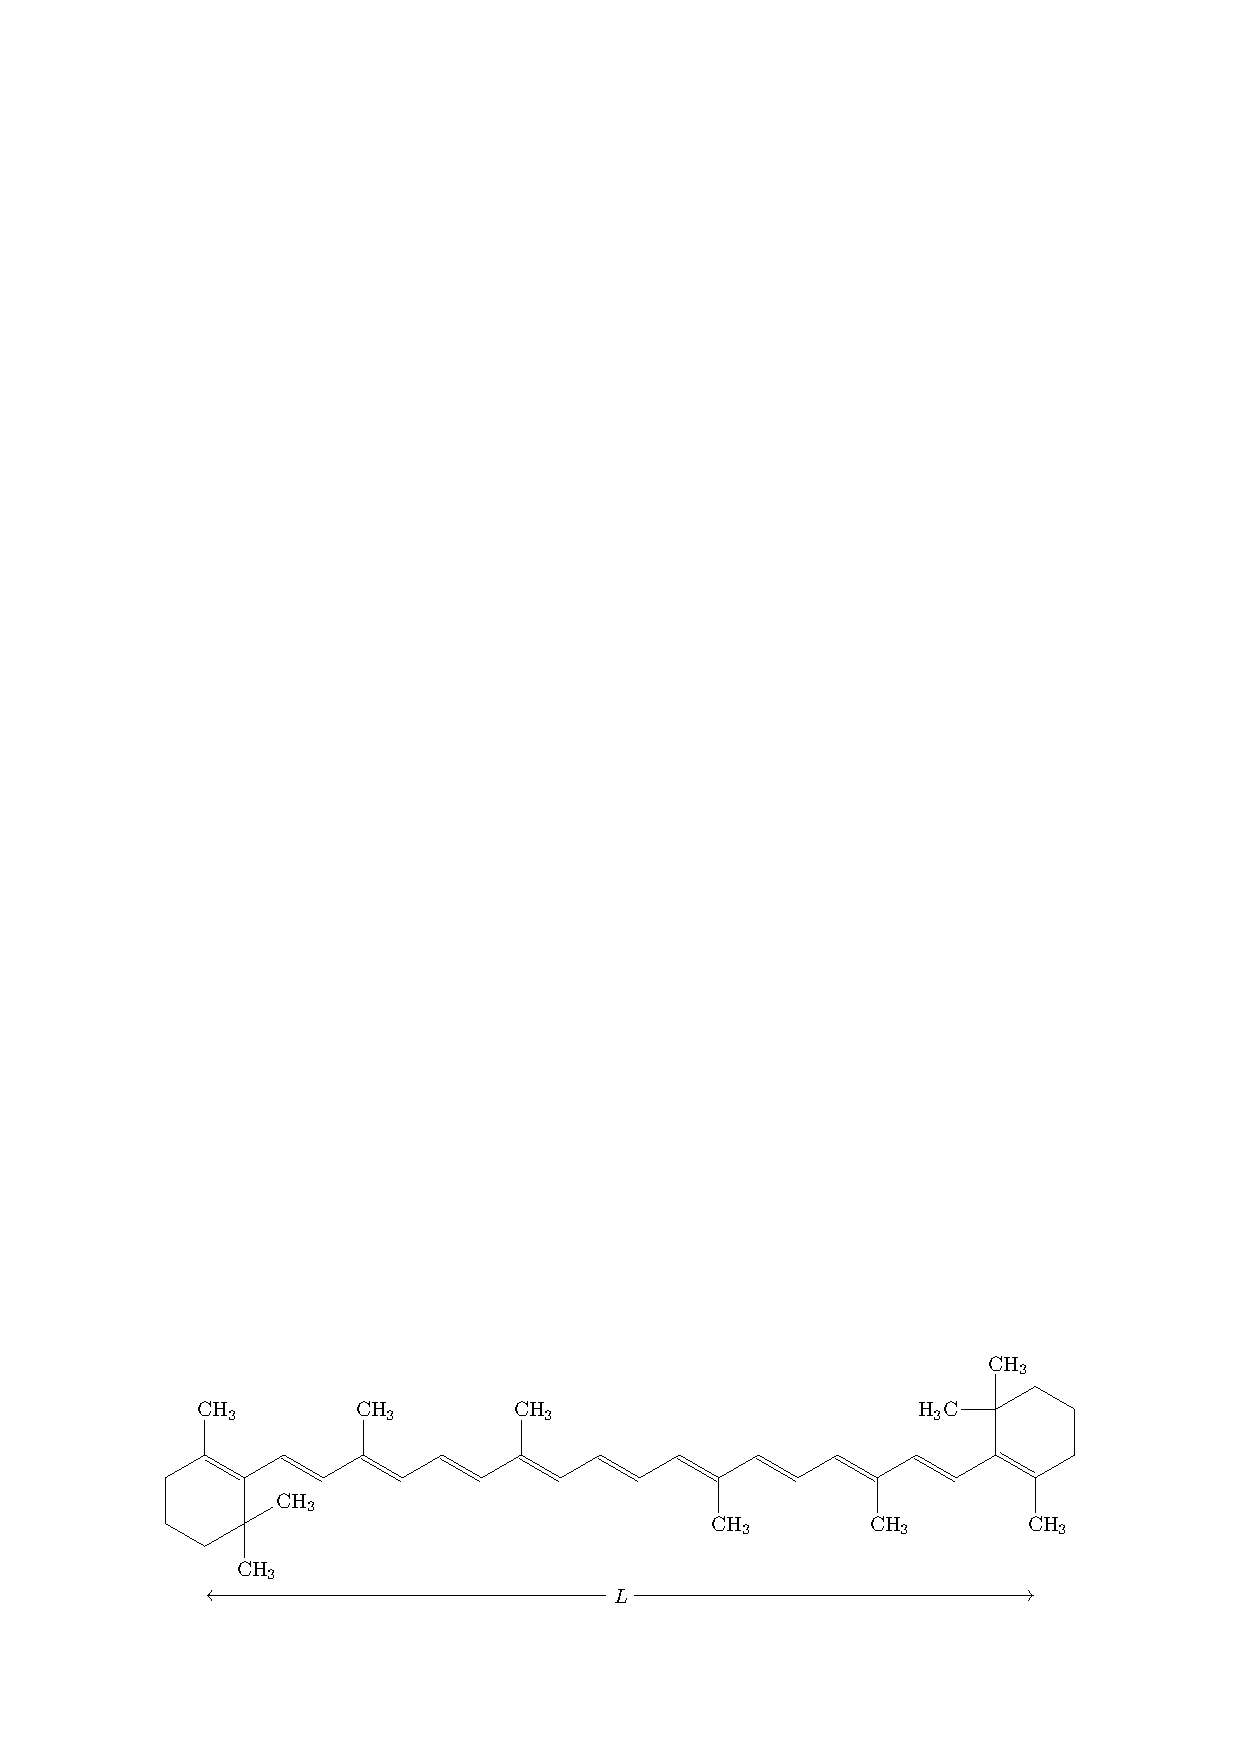
\includegraphics[]{dm7fig/betacarotene.pdf}
	\captionof{figure}{Formule topologique de la molécule de $\beta$-carotène.}
	\label{fig:fig3}
\end{center}

On modélise l'un de ces électrons, de masse $m_\text e$, comme une particule quantique libre de se déplacer le long d'un segment de droite de longueur $L = \SI{1.8}{\nano\meter}$ dont elle ne peut pas sortir. Sa fonction d'onde $\Psi(x)$, indépendante du temps, est alors liée à son énergie $E$ par l'équation dite de Schrödinger, qui prend ici la forme stationnaire suivante :
%
\begin{equation}
    - \dfrac{\hbar^2}{2m_\text e} \dfrac{\dif^2 \Psi}{\dif x^2} = E\Psi \qquad\text{où} \ \hbar = \dfrac{h}{2\pi} \ \text{est la constante de Planck réduite}
\end{equation}

Dans tout l'exercice, l'étude se fait \textit{à une dimension}.

\begin{enumerate}
    \item En remarquant que l'équation de Schrödinger ci-dessus peut être mise sous la forme canonique d'un oscillateur harmonique, donner la forme générale des fonctions d'onde qui en sont solutions. On introduira la pulsation spatiale $k$, dont on donnera l'expression en fonction de $E$, $\hbar$ et $m_\text e$.
    
    \boxans{
        L'équation se réécrit $-\dfrac{\dif^2 \Psi}{\dif x^2} = \dfrac{2Em_\text e}{\hbar^2}\Psi$ puis $\dfrac{\dif^2 \Psi}{\dif x^2} + \dfrac{2Em_\text e}{\hbar^2} \Psi = 0$. On pose $k = \dfrac{\sqrt{2Em_\text e}}{\hbar}$, donc $\dfrac{\dif^2 \Psi}{\dif x^2} + k^2\Psi = 0$.
        
        On reconnaît bien la forme homogène canonique d'un oscillateur harmonique, de solution :
        %
        \[ \Psi(x) = A\sin{kx} + B\cos{kx} \qquad\text{où} \ A \et B \ \text{sont des constantes à déterminer}\]
    }
    
    \item On note $\lambda$ la longueur d'onde associée à la pulsation spatiale $k$. En admettant que l'énergie $E$ de l'électron est uniquement une énergie cinétique, montrer que $\lambda$ correspond à la longueur d'onde de de Broglie de l'électron.
    
    \boxans{
        Par définition on a $k = \dfrac{2\pi}{\lambda}$ donc $\lambda = \dfrac{2\pi}{k} = \dfrac{2\pi\hbar}{\sqrt{2Em_\text e}} = \dfrac{h}{\sqrt{2Em_\text e}}$. Or par hypothèse, l'énergie $E$ de l'électron est uniquement une énergie cinétique, donc $E = \frac{1}{2}m_\text{e}v^2$ ce qui donne bien $\lambda = \dfrac{h}{\sqrt{2\frac{1}{2}m_\text{e}^2v^2}} = \dfrac{h}{m_\text e v} = \dfrac{h}{p} = \lambda_\text{dB}$.
    }
    
    \item Décrire l'interprétation probabiliste associée à la fonction d'onde, et s'en servir pour justifier que $\Psi(x)$ est nulle pour $x$ en dehors de $\left]0, L\right[$.
    
    \boxans{
        La probabilité $\bdP(x)$ de trouver l'électron à la position $x$ est proportionelle à $\mod{\Psi(x)}^2$, donc il existe un $k \in \bdRp$ tel que pour toute position $x$, $\bdP(x) = k\mod{\Psi(x)}^2$. Or il est impossible de trouver la particule pour $x \not\in\left]0, L\right[$, donc pour un tel $x$ on a $\bdP(x) = 0$, donc $k\mod{\Psi(x)}^2 = 0$, donc $\mod{\Psi(x)}^2 = 0$, donc $\Psi(x) = 0$. 
    }
    
    \item On admet que la fonction d'onde doit être continue, et est donc également nulle aux deux extrémités de la molécule. En déduire qu'elle est de la forme
    
    \begin{equation}
        \Psi_n(x) = A_n\sin{\dfrac{n\pi x}{L}}
    \end{equation}
    
    où $n$ est un entier dont on précisera l'ensemble auquel il appartient.
    
    \boxans{
        On sait que $\Psi(x) = A\sin{kx} + B\cos{kx}$. Or $\Psi(0) = 0$ et $\Psi(0) = B$, donc $B = 0$. De plus $\Psi(L) = 0$, donc on a $A\sin{kL} = 0$. $A$ ne peut pas être nul, car l'électron est forcément présent pour $x \in \left[0, L\right]$. Donc $\sin{kL} = 0$. Ainsi il existe $n \in \bdZ$ tel que $kL = n\pi$, donc $k = \dfrac{n\pi}{L}$. Donc $\Psi(x) = A\sin{\dfrac{n\pi x}{L}}$. Il n'y a \textit{a priori} pas de raison que la valeur de $A$ soit la même pour différentes valeurs de $n$, ainsi on obtient bien $\Psi_n(x) = A_n\sin{\dfrac{n\pi x}{L}}$.
    }
\end{enumerate}

À une dimension, la condition de normalisation pour $\Psi_n$ s'écrit

\begin{equation}
    1 = \int_0^L \mod{\Psi_n(x)}^2\;\dif x
\end{equation}

\begin{enumerate}[resume]
    \item Déterminer l'expression de $\mod{A_n}$ en fonction de $L$, et en déduire la dimension de $\Psi_n(x)$.
    
    \boxans{
        On a $\displaystyle \int_0^L \mod{\Psi_n(x)}^2\;\dif x = \mod{A_n}^2\int_0^L \sin^2\left(\dfrac{n\pi x}{L}\right)\dif x =\dfrac{\mod{A_n}^2 L}{n\pi} \int_0^{n\pi} \sin^2\left(t\right)\dif t = \dfrac{\mod{A_n}^2 L}{n\pi}\left[\dfrac{t}{2}-\dfrac{\sin{2t}}{4}\right]_0^{n\pi}$.
        
        Donc $1 = \dfrac{\mod{A_n}^2L}{2}$, d'où $\mod{A_n} = \sqrt{\dfrac{2}{L}}$. On remarque que $\mod{A_n}$ ne dépend pas de $n$.
    }
\end{enumerate}

La fonction d'onde étant déterminée, on peut calculer les énergies possibles que peut prendre l'électron.

\begin{enumerate}[resume]
    \item Montrer que l'électron décrit par la fonction d'onde $\Psi_n$ a une énergie
    
    \begin{equation}
        E_n = \dfrac{\hbar^2 \pi^2}{2m_\text e L^2} n^2
    \end{equation}
    
    \boxans{
        L'énergie $E$ ne provenant par hypothèse que de l'énergie cinétique, on peut évaluer
        %
        \[E = \dfrac{1}{2}m_\text e v^2 = \dfrac{1}{2}m_\text e \left(\dfrac{h}{m_\text e \lambda_\text{dB}}\right)^2 = \dfrac{h^2}{2m_\text e \lambda^2} = \left(\dfrac{h}{2\pi}\right)^2\dfrac{k^2}{2m_\text e} = \dfrac{\hbar^2n^2\pi^2}{2m_\text e L^2} \qquad\text{donc}\qquad E_n = \dfrac{\hbar^2 \pi^2}{2m_\text e L^2} n^2\]
    }
\end{enumerate}

Dans le $\beta$-carotène, ce sont les électrons des onze liaisons doubles qui se comportent comme des particules libres confinées. Ainsi, lorsque les électrons de la molécule sont au repos, ils occupent les onze plus bas niveaux d'énergie. On s'intéresse à l'absorption d'un photon par un électron, faisant passer ce dernier du 11\textsuperscript{e} au 12\textsuperscript{e} niveau d'énergie.

\begin{enumerate}[resume]
    \item Calculer la variation d'énergie d'un électron nécessaire à ce changement de niveau.
    
    \boxans{
        On a $\Delta E = E_{12} - E_{12} = \dfrac{\hbar^2 \pi^2}{2m_\text e L^2}\left(12^2 - 11^2\right) = 23\dfrac{\hbar^2 \pi^2}{2m_\text e L^2}$. L'application numérique donne $\Delta E = \SI{4.3e-19}{\joule}$.
    }
    
    \item En utilisant les relations de Planck-Einstein, calculer la longueur d'onde du photon ainsi absorbé.
    
    \boxans{
        La relation de Planck-Einstein sur le photon $\gamma$ absorbé donne $\Delta E = h \nu = \dfrac{hc}{\lambda_\gamma}$. Donc $\lambda_\gamma = \dfrac{hc}{\Delta E}$. On ré-injecte l'expression de $\Delta E$ et on simplifie, pour obtenir $\lambda_\gamma = \dfrac{8cm_\text e L^2}{23h}$. L'application numérique livre $\lambda_\gamma = \SI{4.6e-7}{\m}$, soit environ $\SI{460}{\nano\m}$.
    }
    
    \item Utiliser ce résultat pour expliquer pourquoi le jus d'orange d'Albert est orange.
    
    \boxans{
        \definecolor{localblue}{RGB}{0, 102, 255}
        \definecolor{localorange}{RGB}{255, 153, 0}
        
        La couleur qui correspondant à une longueur d'onde de $\SI{460}{\nano\m}$ est un bleu cyan. On suppose que le verre de jus d'orange est éclairé par une lumière blanche. La couleur complémentaire est alors le orange, ce qui explique la couleur du jus. Plus précisément, en s'appuyant sur le programme de Dan Bruton (\href{http://www.physics.sfasu.edu/astro/color/spectra.html}{\texttt{www.physics.sfasu.edu/astro/color/spectra.html}}), on obtient qu'une telle longeur d'onde correspond environ à \SI{0}{\percent} de rouge, \SI{40}{\percent} de vert et \SI{100}{\percent} de bleu, soit \fcolorbox{black}{localblue}{\rule{0pt}{4pt}\rule{15pt}{0pt}}. En supposant que le verre est éclairé par une lumière blanche, la couleur du jus correspond alors à \SI{100}{\percent} de rouge, \SI{60}{\percent} de vert et \SI{0}{\percent} de rouge, soit \fcolorbox{black}{localorange}{\rule{0pt}{4pt}\rule{15pt}{0pt}}. On retrouve bien une couleur orange.
    }
    
    
\end{enumerate}

\section{Albert se brosse les dents}

Satisfait de son petit-déjeuner, et avant de se rendre à son laboratoire de recherche, Albert retourne dans la salle de bain pour se laver les dents.\\[2pt]
%
Dans une salle de bain, l'eau est délivrée par deux types de robinets : le mitigeur mécanique pour les lavabos et le mitigeur thermostatique pour la douche ou la baignoire.

\begin{center}
    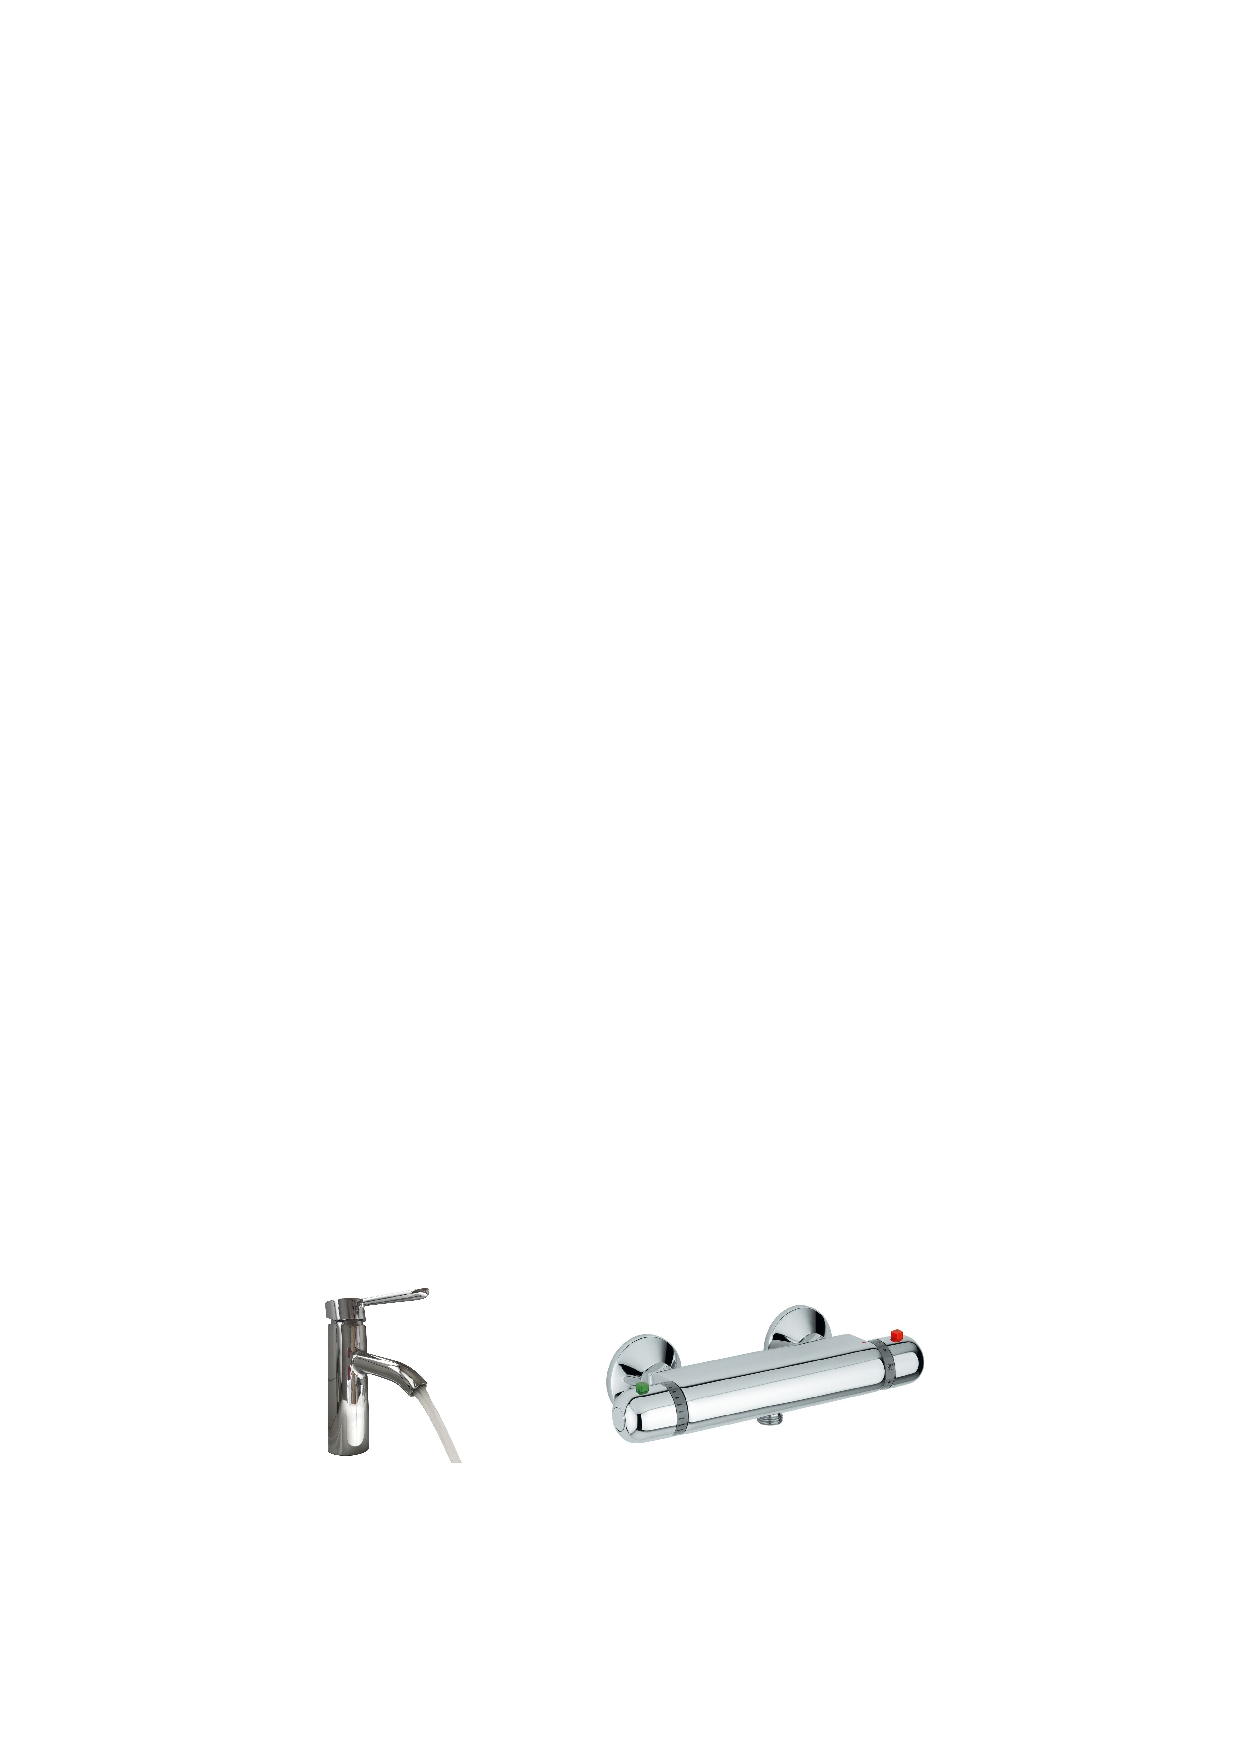
\includegraphics[]{dm7fig/mitigeursex.pdf}
	\captionof{figure}{Exemples de mitigeurs, mécanique à gauche et thermostatique à droite.}
	\label{fig:fig4}
\end{center}

Dans le mitigeur mécanique, l'eau froide et l'eau chaude sont mélangées dans des proportions réglables par une position angulaire de la poignée et le débit réglable indépendamment par l'inclinaison de la poignée. L'écoulement est étudié en régime stationnaire et on note $D_\text C$ et $D_\text F$ les débits massiques respectifs de l'eau chaude (température $T_\text C$) et de l'eau froide (température $T_\text F$) à l'entrée dans le mélangeur et $D_\text S$ le débit massique de l'eau en sortie (température $T_\text S$).\\[2pt]
%
On suppose que la capacité thermique massique de l'eau, notée $c_\text e$, est indépendante de sa température.

\begin{enumerate}
    \item Parmi les quatre valeurs proposées ci-dessous, quel débit $D_\text S$ en sortie du mitigeur correspond à un fonctionnement normal ? Argumenter.
    
    \begin{enumerate}
        \begin{minipage}{0.25\textwidth}
            \itt $\SI{2.0}{\g \cdot \second^{-1}}$
        \end{minipage}
        %
        \begin{minipage}{0.25\textwidth}
            \itt $\SI{2.0e1}{\g \cdot \second^{-1}}$
        \end{minipage}
        %
        \begin{minipage}{0.25\textwidth}
            \itt $\SI{2.0e2}{\g \cdot \second^{-1}}$
        \end{minipage}
        %
        \begin{minipage}{0.25\textwidth}
            \itt $\SI{2.0e3}{\g \cdot \second^{-1}}$
        \end{minipage}
    \end{enumerate}
    
    \boxans{
        La masse volumique de l'eau est $\rho = \SI{1.0}{\g \cdot \mL}$. Ne recevoir que $\SI{2.0}{\mL}$ d'eau par seconde semble peu pour prendre une utilisation normale. Recevoir $\SI{1.0}{\L}$ toutes les $5$ secondes, ou toutes les demi-secondes semble par ailleurs trop élevé, il s'agit donc de la deuxième valeur : $D_\text S =\SI{2.0e1}{\g \cdot \second^{-1}} $.
    }
    
    \item Relier $D_\text S$ à $D_\text F$ et $D_\text C$.
    
    \boxans{
        L'eau en sortie correspond au mélange de l'eau froide et de l'eau chaude, donc $D_\text S = D_\text C + D_\text F$.
    }
    
    \item Est-il légitime de faire l'hypothèse que l'eau dans le corps du mélangeur ne reçoit aucune puissance thermique de la part de l'air environnant ?
    
    \boxans{
        Le robinet sépare l'eau dans le corps du mélange de l'air environnant, et se comporte comme un isolant thermique. L'air de plus, à cette échelle (taille et temps, l'eau du robinet étant renouvelée rapidement), est un mauvais conducteur thermique. On peut donc supposer que le robinet agit comme une paroi adiabatique. L'eau dans le corps du mélangeur ne reçoit donc aucune puissance thermique de la part de l'air environnant.
    }
\end{enumerate}

On peut montrer que
%
\begin{equation}
    D_\text S h_\text S = D_\text C h_\text C + D_\text F h_\text F
\end{equation}

où $h_\text S$, $h_\text C$ et $h_\text F$ sont les enthalpies massiques respectives de l'eau en sortie, chaude et froide.

\begin{enumerate}[resume]
    \item En admettant que l'eau vérifie la seconde loi de Joule, montrer que
    
    \begin{equation}
        T_\text S = \dfrac{D_\text C T_\text C + D_\text F T_\text F}{D_\text C + D_\text F}
    \end{equation}
    
    \boxans{
        On a $D_\text S h_\text S = D_\text C h_\text C + D_\text F h_\text F$, d'où $h_\text S = \dfrac{D_\text C h_\text C + D_\text F h_\text F}{D_\text S}$. On suppose la seconde loi de Joule, donc $h_\text i = c_\text e T_\text i$ d'où $c_\text eT_\text S = \dfrac{D_\text C c_\text eT_\text C + D_\text F c_\text eT_\text F}{D_\text S}$. On divise par $c_\text e$ pour obtenir $T_\text S = \dfrac{D_\text C T_\text C + D_\text F T_\text F}{D_\text C + D_\text F}$.
    }
\end{enumerate}

La légionellose est une maladie infectieuse due à une bactérie qui se développe dans les réseaux d'eau douce dont la température est comprise entre $\SI{25}{\celsius}$ et $\SI{45}{\celsius}$. À $\SI{50}{\celsius}$, sa croissance est stoppée, mais la bactérie survit ; à $\SI{55}{\celsius}$, le temps de destruction est de plusieurs heures, à $\SI{50}{\celsius}$ il est de 32 minutes, à $\SI{70}{\celsius}$ de une minute. Dans les logements où la production d'eau chaude est individuelle, il est donc recommandé de maintenir l'eau du ballon de stockage à une température de plus de $\SI{55}{\celsius}$ et une fois par semaine de produire une eau à $\SI{70}{\celsius}$. La température d'eau chaude à l'arrivée au robinet doit être au moins de $\SI{50}{\celsius}$.\\[2pt]
%
La gravité d'une brûlure est fonction de la température de l'eau et du temps de contact avec la peau. Une brûlure au troisième degré survient lors d'une exposition de la peau d'une seconde à $\SI{70}{\celsius}$, 7 secondes à $\SI{60}{\celsius}$ et 8 minutes à $\SI{50}{\celsius}$.\\[2pt]
%
Un mitigeur mécanique est réglé pour que la température de sortie soit de $\SI{42}{\celsius}$ lorsque $T_\text C = \SI{50}{\celsius}$ et $T_\text F =\SI{18}{\celsius}$. La manette est alors abaissée en position robinet fermé. Durant la nuit, l'eau chaude sanitaire est produite à une température de $\SI{70}{\celsius}$.

\begin{enumerate}[resume]
    \item Y a-t-il un risque de brûlure à l'ouverture du mitigeur le matin si Albert lève simplement la manette sans la tourner ni à gauche ni à droite ?
    
    \boxans{
        Le mitigeur mécanique étant réglé pour que la température de sortie soit de $T_\text S = \SI{42}{\celsius}$ lorsque $T_\text C = \SI{50}{\celsius}$ et $T_\text F =\SI{18}{\celsius}$, on peut calculer $D_\text F$ à partir de $T_\text S = \dfrac{\left(D_\text S - D_\text F\right) T_\text C + D_\text F T_\text F}{D_\text S}$, soit $D_\text F = D_\text S \dfrac{T_\text S - T_\text C}{T_\text F - T_\text C}$. L'application numérique donne $D_\text F = \SI{5.0}{g \cdot \second^{-1}}$ On calcule alors $D_\text C = D_\text S - D_\text F = \SI{15}{g \cdot \second^{-1}}$. On suppose qu'au matin l'eau chaude est toujours de température $T'_\text C = \SI{70}{\celsius}$. On calcule alors la température de sortie $T'_\text S = \dfrac{D_\text C T'_\text C + D_\text F T_\text F}{D_\text C + D_\text F}$. L'application numérique donne $T'_\text S = \SI{57}{\celsius}$. La durée étant de $7$ seconde pour $\SI{60}{\celsius}$ et de 8 minutes  $\SI{50}{\celsius}$, elle devrait valoir par moyenne géométrique environ une minute. Albert devrait donc avoir le temps de réagir avant de se bruler.
    }
\end{enumerate}

Un mitigeur thermostatique contient un élément dilatable, par exemple une cartouche de cire. Si la température de l'eau chaude augmente brusquement, la régulation de température de l'eau de sortie est alors effectuée sans agir sur le
réglage de la manette.

\begin{enumerate}[resume]
    \item L'eau chaude arrive-t-elle sur l'entrée 1 ou l'entrée 2 du schéma de la figure \ref{fig:fig5} ? Justifier.
    
    \boxans{
        L'eau chaude est principalement susceptible de changer brusquement de température (bien plus que l'eau froide). Il s'agit donc de faciliter la réaction de la cire avec ce changement, et donc de maximiser son \guill{interaction} avec l'eau chaude. Bien sûr, si l'eau chaude change brusquement de température, le mélange (en contact direct avec la cire) le fera aussi. Toutefois faire passer l'eau chaude par l'entrée 2 maximise son contact la vis qui passe par la cire dilatable, et agirait donc comme conducteur thermique.
    }
\end{enumerate}

\begin{center}
    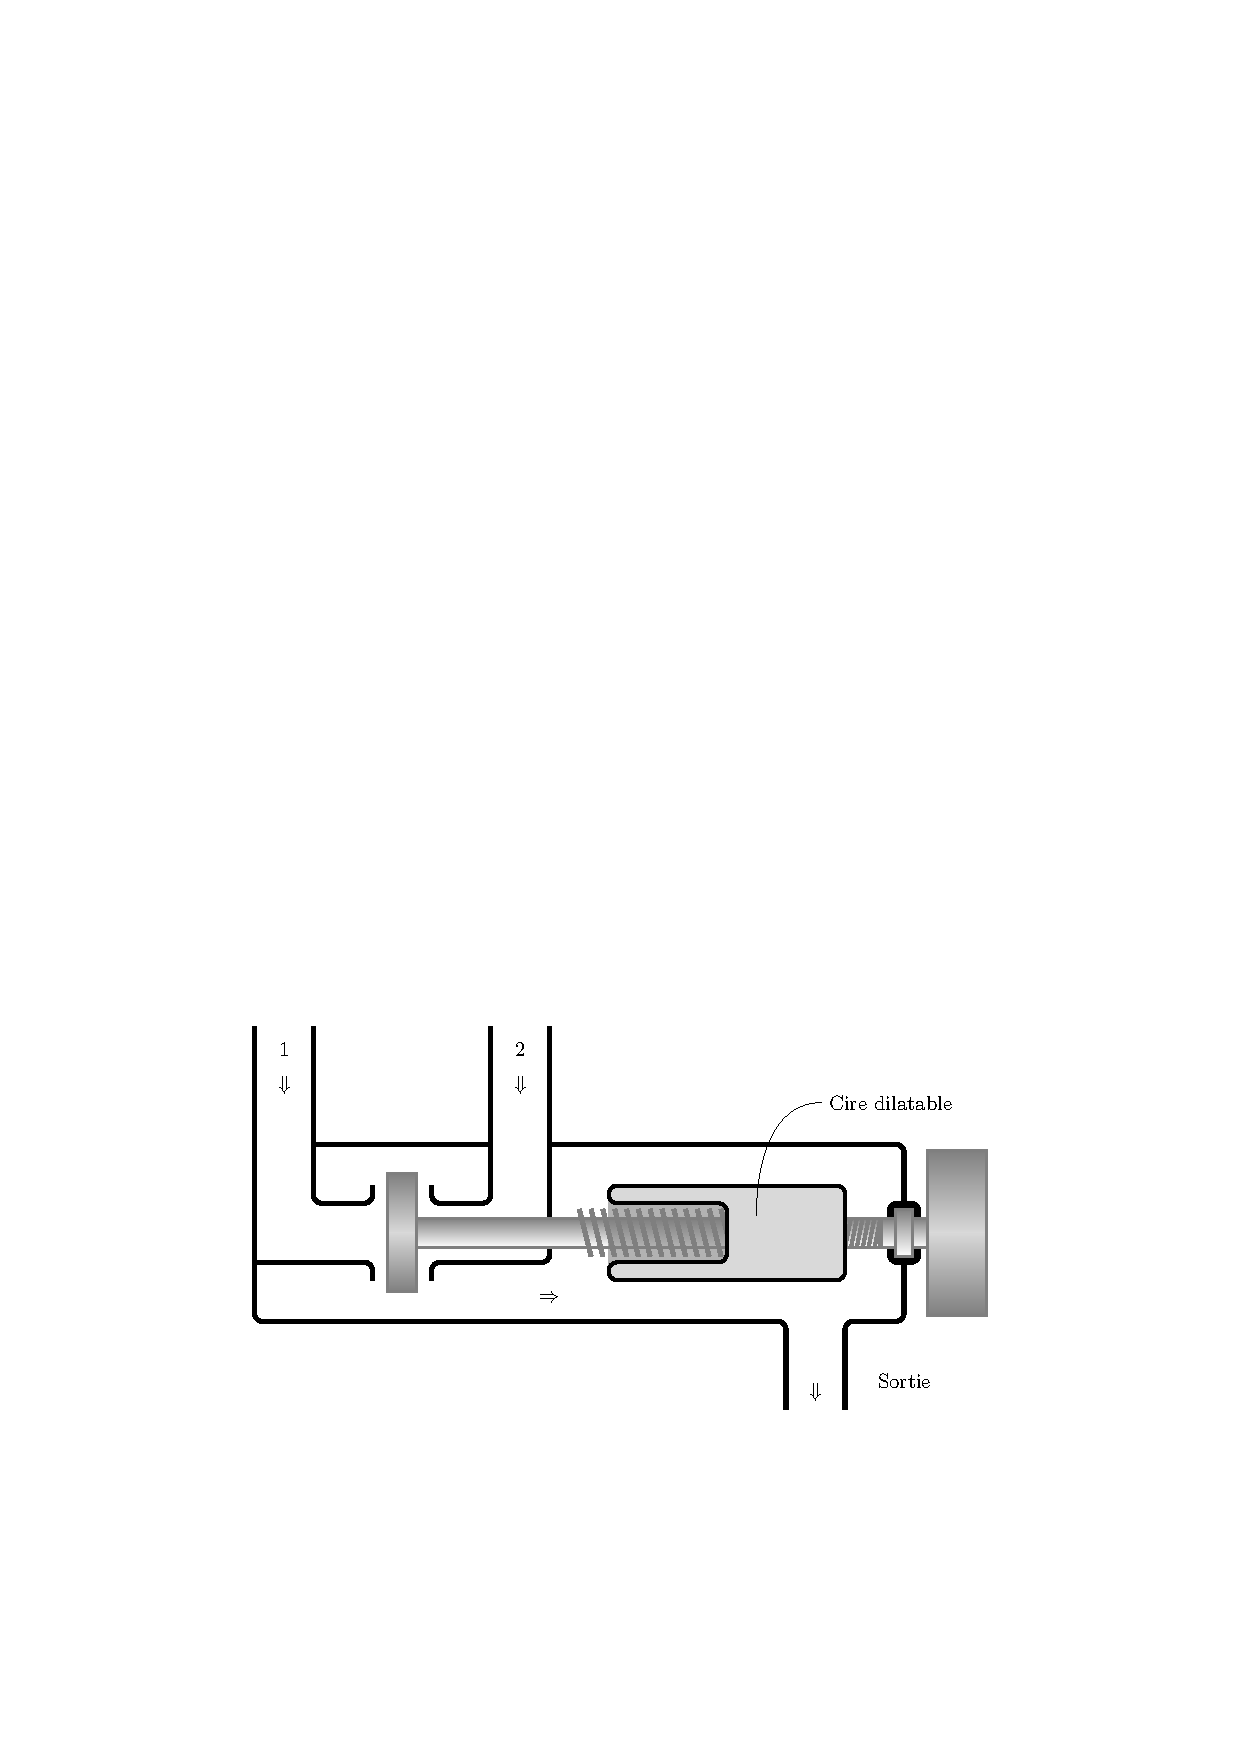
\includegraphics[]{Physique/DM/dm7fig/mitigeurschem.pdf}
	\captionof{figure}{Mitigeur thermostatique schématique.}
	\label{fig:fig5}
\end{center}


\end{document}